% -----------------------------------------------------------------------------
% June 1, 2016
% This file contains a sample Bridges paper in LaTeX format.
% It has been prepared by Doug McKenna, using previous
% versions by Craig Kaplan, Reza Sarhangi, and others.
% It has been vetted using TeXShop 2.36 on Mac OS X (10.6).
% TeXShop is part of the TeX Live distribution, available
% at http://www.tug.org/texlive/
%
% -----------------------------------------------------------------------------

\documentclass[11pt]{article}
\usepackage{amsmath, amsthm, amssymb}    % May not all be necessary
\usepackage{bridges}                     % Custom bridges proceedings style
\usepackage{graphicx}                    % For including pictures
\usepackage{hyperref}                    % For formatting (clickable) URLs
\usepackage{subcaption}		     % Aaron added this one for certain figures

% -----------------------------------------------------------------------------

\title{Seeing and Hearing the Eigenvectors of a Fluid}
\author{ Aaron Demby Jones, JoAnn Kuchera-Morin and Theodore Kim\\
Media Arts and Technology Program\\ University of California, Santa Barbara\\
{\tt aaron.demby.jones@mat.ucsb.edu, jkm@create.ucsb.edu, kim@mat.ucsb.edu}
}
% TK: MAT is a Program, not a Department. On my side, this is an MAT project, not a Pixar project.

% \date{[Draft as of \today]}	% For your own draft purposes
\date{}				% Suppress any date on submissions

% -----------------------------------------------------------------------------

\begin{document}

% -----------------------------------------------------------------------------
% Aaron's convenience commands
\newcommand{\UU}{\mathbf{U}}
\newcommand{\uu}{\mathbf{u}}
\newcommand{\vv}{\mathbf{v}}
\newcommand{\utilde}{\mathbf{q}}
\newcommand{\ff}{\mathbf{f}}
\newcommand{\qq}{\mathbf{q}}
\newcommand{\aaa}{\mathbf{a}}
\newcommand{\R}{\mathbb{R}}
\newcommand{\subspace}{\mathbb{S}}
\newcommand{\boldA}{\mathbf{A}}
\newcommand{\VV}{\mathbf{V}}
% -----------------------------------------------------------------------------
% Ted's commands
\newcommand{\todo}[1]{$\spadesuit$ {\bf #1} $\spadesuit$}


\maketitle

% Prevent page number 1 from being printed on the first page.
\thispagestyle{empty}

\begin{abstract}
The intricate shapes and sounds that arise from the eigenvectors of vibrating Chladni plates are a well-known phenomenon. We explore a generalization of this phenomenon by computing the patterns formed by the empirical eigenvectors of a computational fluid dynamics simulation. The eigenvectors form abstract, turbulent patterns in space, especially in the presence of non-physical excitations. The eigenvalues form a spectrum that does not possess a unique sonic mapping, so we construct a sonification that allows us to listen to the trajectory of the fluid.
\end{abstract}

% Bridges papers are usually no more than 8 pages in length.  So
% there's really no need to have numbered sections, unless the
% author really needs to refer to sections within the paper's text.  So to suppress
% sequential section numbers, append an asterisk to the \section command, as in:

%%%%%%%%%%%%%%%%%%%%%%%%%%%%%%%%%%%%%%%%%%%
\section*{Introduction}
Chladni plates beautifully reveal the vibration modes, also known as the eigenvectors, of a rigid plate (Fig.~\ref{fig:chladni-plate}). These eigenvectors can be computed analytically, as they correspond to very small deformations (i.e.~vibrations) on a very simple domain, and can be written in terms of the Bi-Laplacian operator $(\Delta^2)$ over a square domain \cite{gander2012euler}. These visual representations can be extended to more complex scenarios, where the eigenvectors and their corresponding eigenvalues are instead computed numerically. In this work, we compute the eigenvectors of a dynamic computational fluid dynamics simulation, which involves large deformations instead of small vibrations, and the Navier-Stokes equations in lieu of a Bi-Laplacian. We then visualize the turbulent motion of the eigenvectors in this spectral representation, and construct a sonification of the resulting frequencies to produce a mapping between fluid trajectories and sound. The results are organic visual forms with a unique visual character, and a variety of associated sounds that unfold over rich spectral envelopes.

\begin{figure}
%\centering
%	\begin{subfigure}[h]{0.4\textwidth}
%		\centering
%		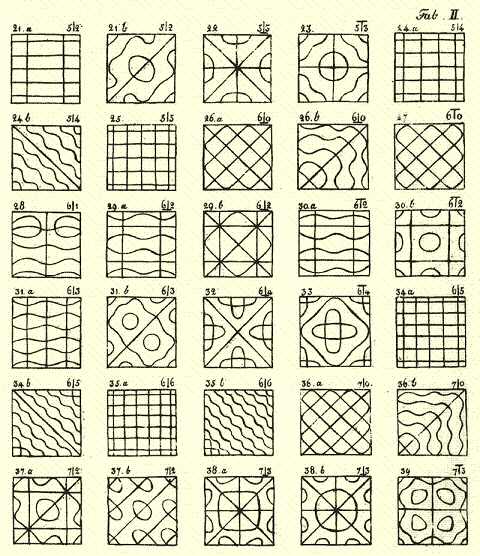
\includegraphics[width=\textwidth]{Figures/chladni_drawing.png}
%		\caption{A table of hand-drawn Chladni figures. Source: Wikimedia Commons.}
%		\label{fig:chladni-drawn}
%	\end{subfigure}
%	%
%	 \hspace{3em}
%	\begin{subfigure}[h]{0.4\textwidth}
%		\centering
%		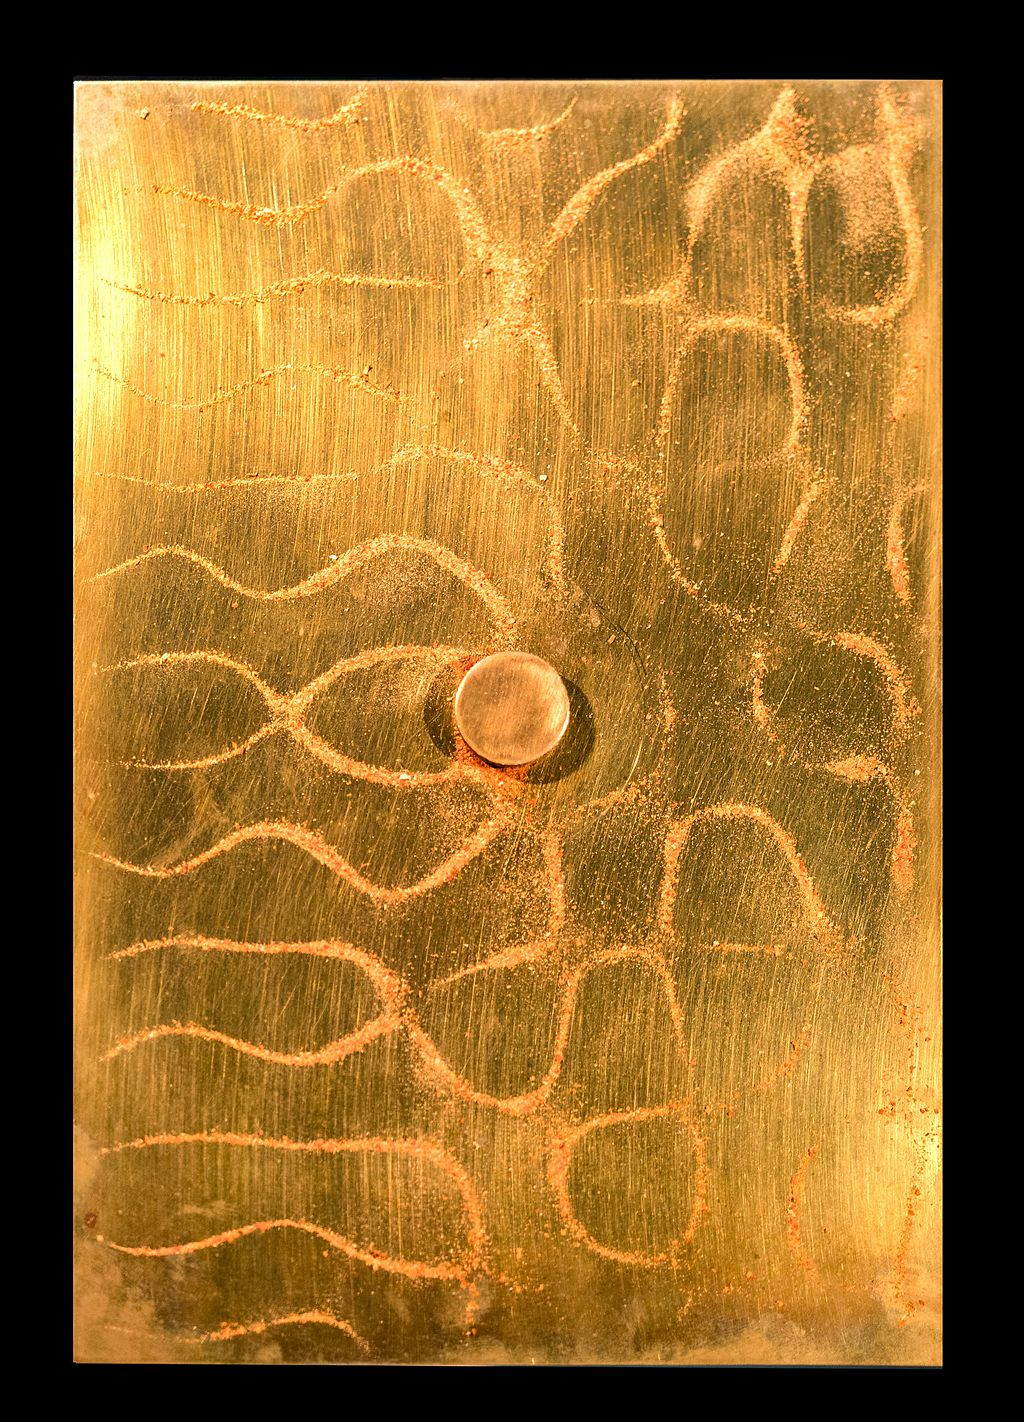
\includegraphics[width=\textwidth]{Figures/chladni_plate.jpg}
%		\caption{The physical experiment with a rectangular plate. Source: Wikimedia Commons.}
%		\label{fig:chladni-plate}
%	\end{subfigure}
%	\caption{Chladni figures, both hand-drawn and experimentally realized.}
		\centering
		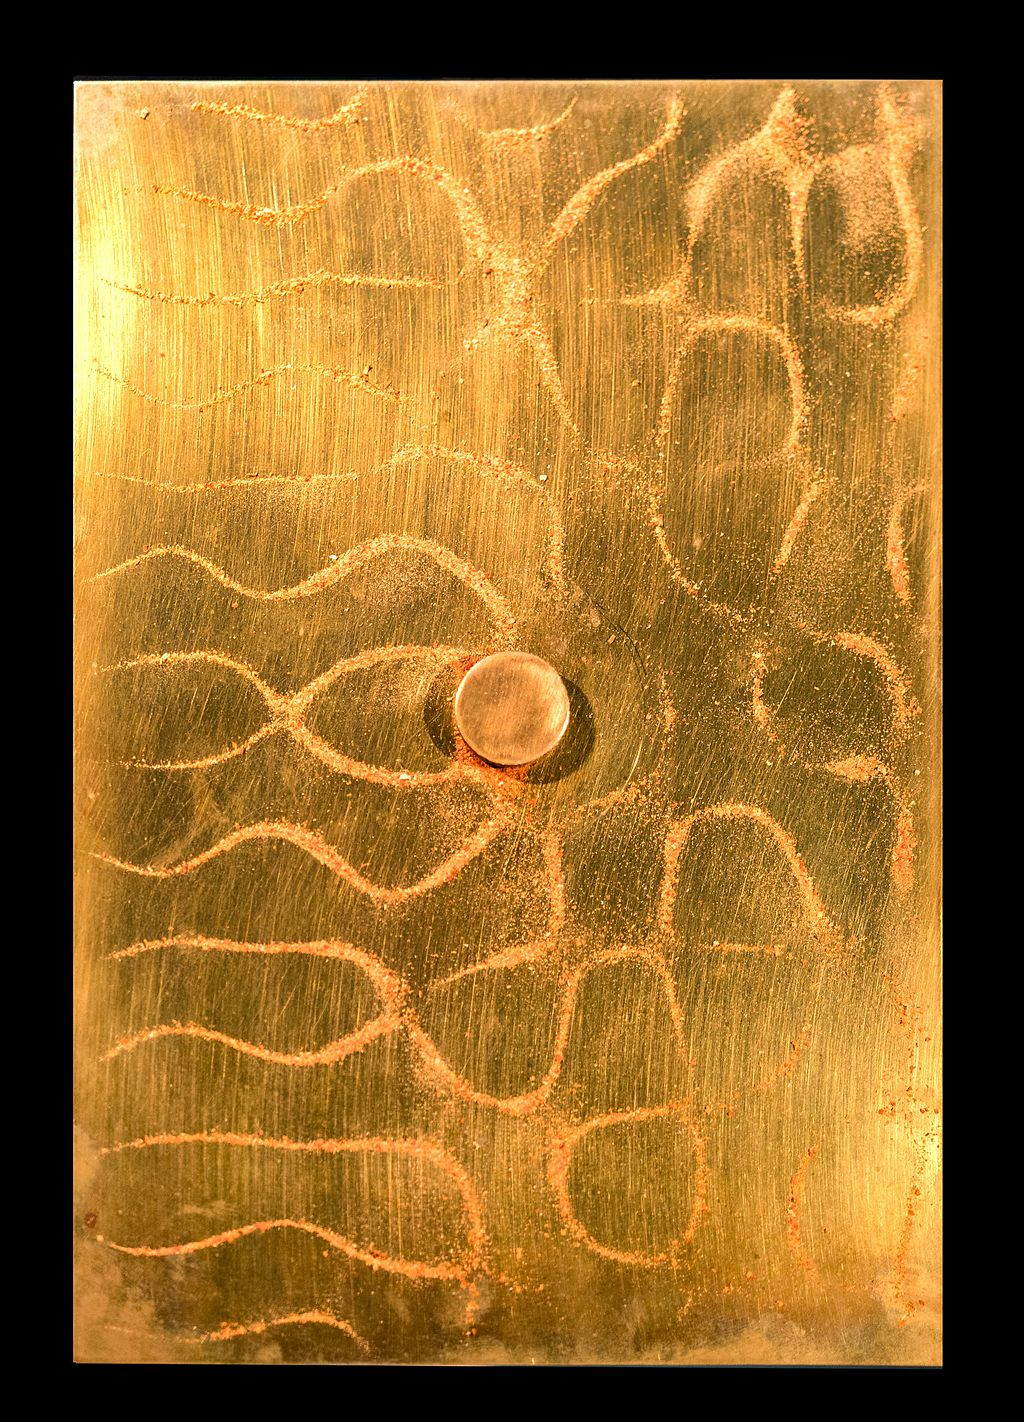
\includegraphics[angle=90,origin=c, width=0.5\textwidth]{Figures/chladni_plate.jpg}
		\vspace*{-2em}
		\caption{Chladni patterns realized through a physical experiment with a rectangular plate. Source: Wikimedia Commons.}
		\label{fig:chladni-plate}
\end{figure}

\section*{Empirical Eigenvectors of a Fluid}

In this work, we would like to compute the eigenvectors that arise from the Navier-Stokes equations for fluid flow. There are several different strategies for computing these vectors. For example, de Witt et al. \cite{deWitt:2012} computed the analytic eigenfunctions of the fluid velocity field over a simple square domain, and used it to advect (i.e.~push around) a particulate through space. These eigenfunctions are composed of separable products of sines and cosines, and the results visually correspond almost directly to classic Chladni patterns. \todo{TK: I suppose I could generate a figure for this}

We are interested in generating less classical results, so we prefer the use of ``empirical'' eigenvectors \cite{Ryckelynck2005}. This approach goes many names, such as Proper Orthogonal Decomposition, Karhunen-Love expansion, or Hotelling transform, but we prefer the eigenvector nomenclature because it clarifies the connection to Chladni patterns. As the name suggests, it involves computing the eigenvectors of an empirically obtained data set, in this case the results of a computational fluid dynamics (CFD) simulation.

The eigenvectors are constructed as follows. We have a velocity field defined on a regular three-dimensional grid of $N$ cells, which we consider abstractly as the real vector space $\R^{3N}$. The CFD simulation has been stepped over $T$ timesteps, so it provides $T$ velocity fields defined over this grid. We would then like to discover the $r$ most important eigenvectors of this data set, $\uu_1, \ldots, \uu_r \in \R^{3N}$. If we arrange the $T$ velocity fields of the CFD simulation into the columns of a matrix, we obtain $\boldA \in \R^{3N \times T}$. Taking the singular value decomposition (SVD) yields $\boldA = \UU \Sigma \VV^T$.

The columns of $\UU$ are our ``empirical'' eigenvectors, and $\Sigma$ is a diagonal matrix of singular values. In some special cases, these values can correspond directly to audio frequencies, but in the general case of arbitrary CFD simulations we are considering, this correspondence is no longer uniquely determined. However, we will later take the sometimes existence of this correspondence as a launching point for our own sonification strategy. As we are only interested in the $r$ most important eigenvectors, we usually truncate $\UU$ to its first $r$ columns, yielding $\UU \in \R^{3N \times r}$.

The columns of $\UU$ comprise an $r$-dimensional subspace $\R^r$ inside of $\R^{3N}$, and $\UU$ itself defines a projection operator. Given the $t$th velocity field from the original CFD simulation $\uu_t \in \R^{3N}$, we can compute a much smaller, ``reduced-order'' approximation of $\uu_t$ by computing $\UU^T \uu_t = \qq_t \in \R^r$. The fact that ``subspace'' coordinates can be constructed in this manner has attracted significant interest in the engineering community, because it is then often possible to run simulations, even those using the full Navier-Stokes equations, very quickly within this coordinate system \cite{Kim2013}. We are interested in this representation for two additional reasons. First, it is straightforward to interpret the entries in each $\qq_t$ as the amplitudes in a quasi-frequency spectrum. Therefore, they are a convenient starting point for constructing a sonic representation of fluid motion. Second, the projection can be reversed, or ``lifted''. Given an arbitrary sound $\qq$ that was constructed in the quasi-frequency spectrum, we can unambiguously translate that sound into a fluid motion by ``lifting'' the vector back to the $\R^{3N}$ space by computing $\UU \qq = \uu$. Therefore, we can use a sound to drive a fluid's motion.

%At each time step $t$, we integrate the equations of motion for $\qq \in S$ to advance forward to $\qq_{t+1} \in S$. Being over a reduced number of variables, this phase is greatly accelerated compared to the full-space integration. Once the integration is complete, we must reverse the projection so that the results can be displayed in the original space of full coordinates. This reconstruction can be achieved simply by computing $\uu_{t+1} = \UU\qq_{t+1}$.
%
%There are several strategies for discovering a useful subspace $S$, both analytical and statistical in nature. In work by de Witt \cite{deWitt:2012} the subspace $S$ is determined analytically by eigenfunctions of the Laplacian operator on a box up to a desired threshold frequency. In previous work by Kim \cite{Kim2013}, the subspace $S$ is statistically discovered by first performing an appropriate training simulation in full coordinates and performing a singular value decomposition over a matrix $A$ whose columns are velocity fields at each time step. Discarding the singular values less than a small threshold leaves us with $r$ singular values, with $r \ll 3N$, and their corresponding $r$ singular vectors, which are the basis vectors in the full space $\R^{3N}$ that generate $S$. In either the analytical or statistical case, in analogy to the Chladni plate vibrations, the singular vectors correspond to the eigenfunctions, and the singular values correspond to the frequencies. Because the eigenfunctions of the Laplacian operator on a box are well-known to be separable products of sine and cosine functions, we use the statistical approach to generating the subspace $S$ in this paper in order to discover more unfamiliar modes.
%    
%For each time step of the subspace re-simulation, when we perform the reconstruction phase, obtaining a full-space velocity field $\vv \in \R^{3N}$ from a reduced-order subspace vector $\qq \in \R^r$, we are simply taking a linear combination of the $r$ singular vectors using the corresponding coefficients given by the entries of $\qq$. Hence, the subspace vectors $q$ can be intuitively thought of as instructions for how to mix together the corresponding singular vectors with the appropriate weightings. Indeed, we can even identify a path $\varphi \colon [0, 1] \rightarrow S$, sampled at $T$ timesteps $\varphi_1, \ldots, \varphi_T$, as determining the corresponding $T$ timesteps of the full-space re-simulation, after reconstruction.

%%%%%%%%%%%%%%%%%%%%%%%%%%%%%%%%%%%%%%%%%%%

\section*{Visualization}
To generate a suitably interesting subspace of possible motions, we generated six separate full-coordinate flows of a single plume of smoke moving toward each of the faces of a bounding box. After performing a singular value decomposition and truncating to $r = 150$ singular values and singular vectors, we obtained the desired subspace $S$. To reveal the shape of the modes, we ran a simulation with each of the modes sequentially isolated; i.e., each subspace vector $q_{t} \in S$ at time step $t$ was the vector with a $1$ in position $t$ and $0$ elsewhere.

%%%%%%%%%%%%%%%%%%%%%%%%%%%%%%%%%%%%%%%%%%%
% ADJ: These are the 'coupled' modes, not as strong an analogy to the Chladni plates.
\begin{figure*}
	\begin{subfigure}[h]{0.5\textwidth}
		\centering
		\includegraphics[width=\textwidth]{Figures/renders/plume0007.png}
	\end{subfigure}
	%	
	\begin{subfigure}[h]{0.5\textwidth}
		\centering
		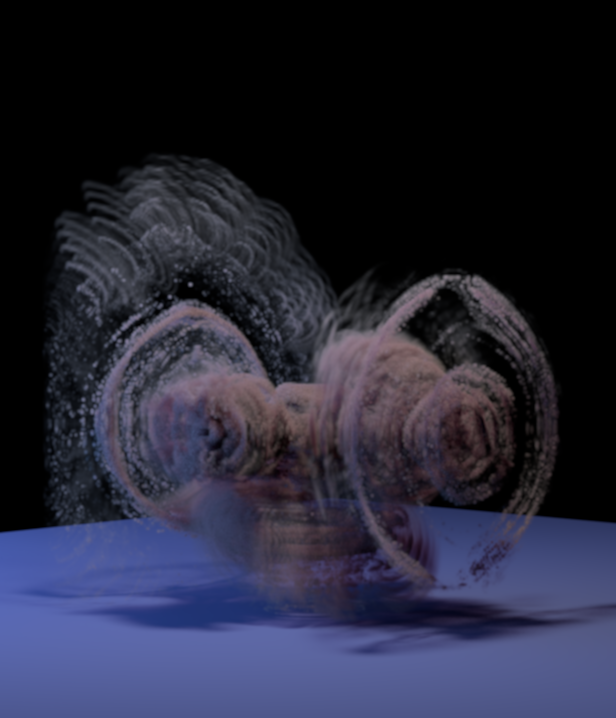
\includegraphics[width=\textwidth]{Figures/renders/plume0008.png}	
	\end{subfigure}
	%
	\begin{subfigure}[h]{0.5\textwidth}
		\centering
		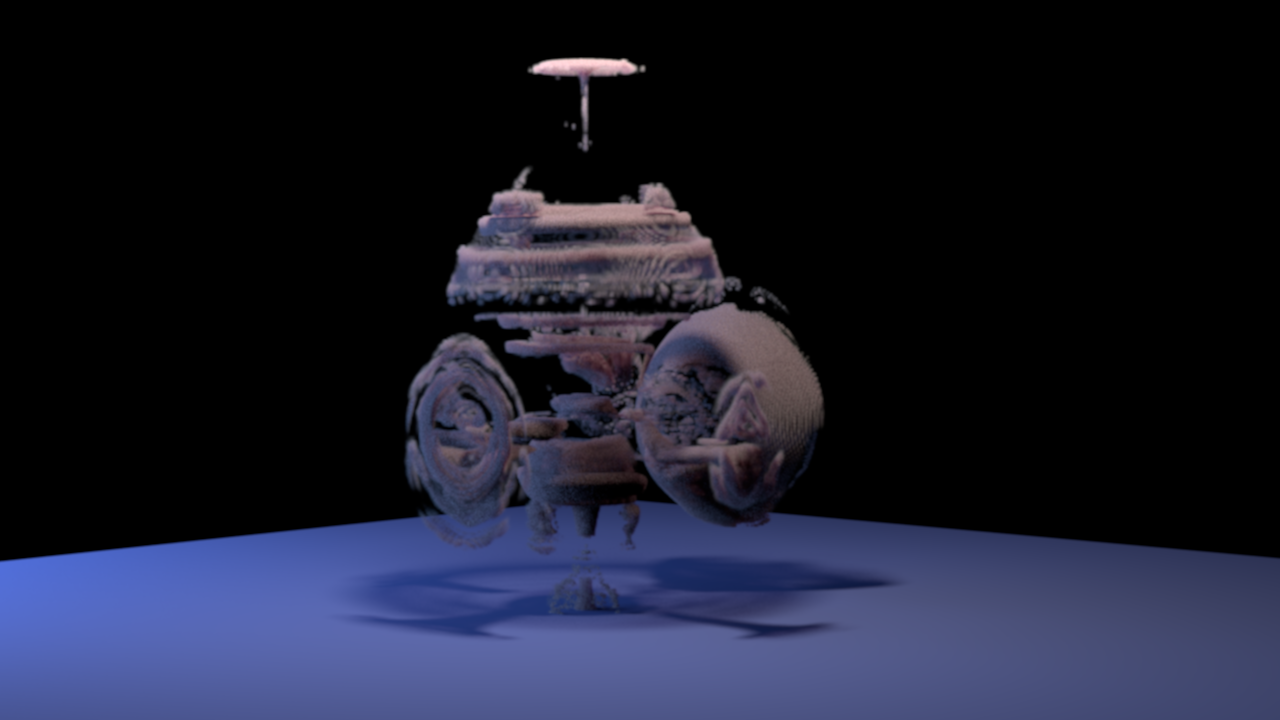
\includegraphics[width=\textwidth]{Figures/renders/plume0009.png}
	\end{subfigure}
	%
	\begin{subfigure}[h]{0.5\textwidth}
		\centering
		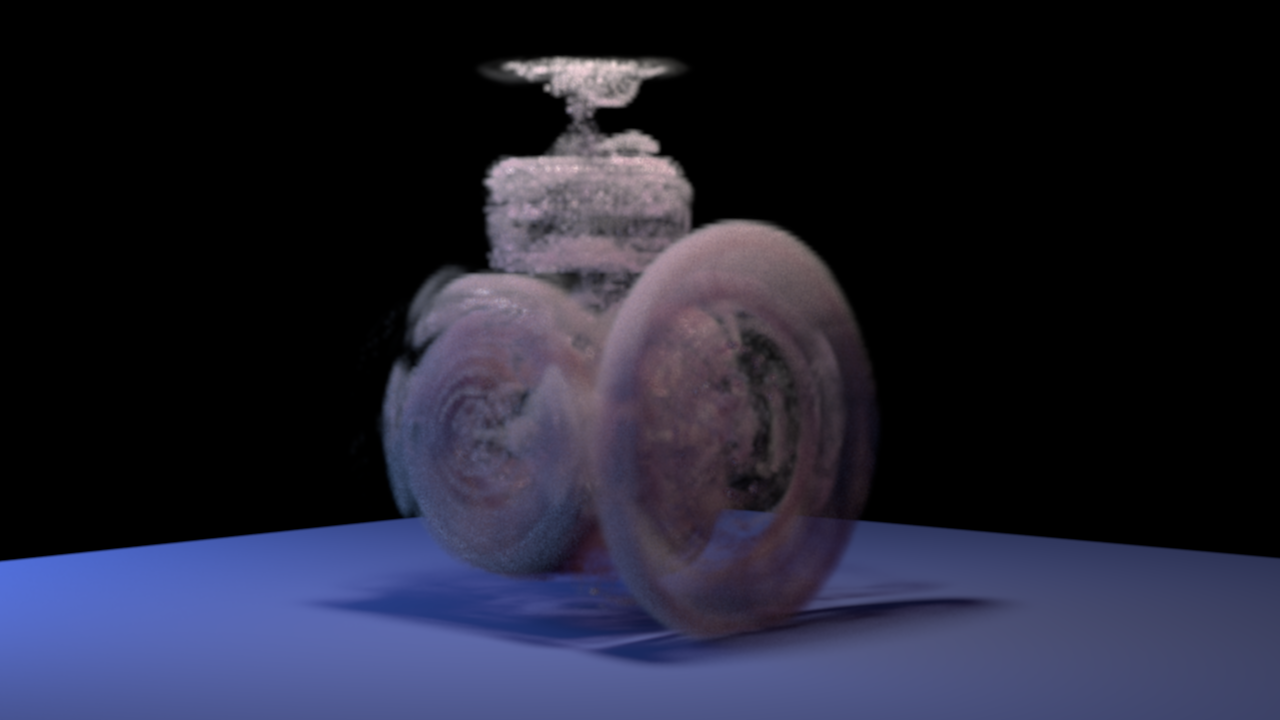
\includegraphics[width=\textwidth]{Figures/renders/plume0014.png}
	\end{subfigure}
	%
	\begin{subfigure}[h]{0.5\textwidth}
		\centering
		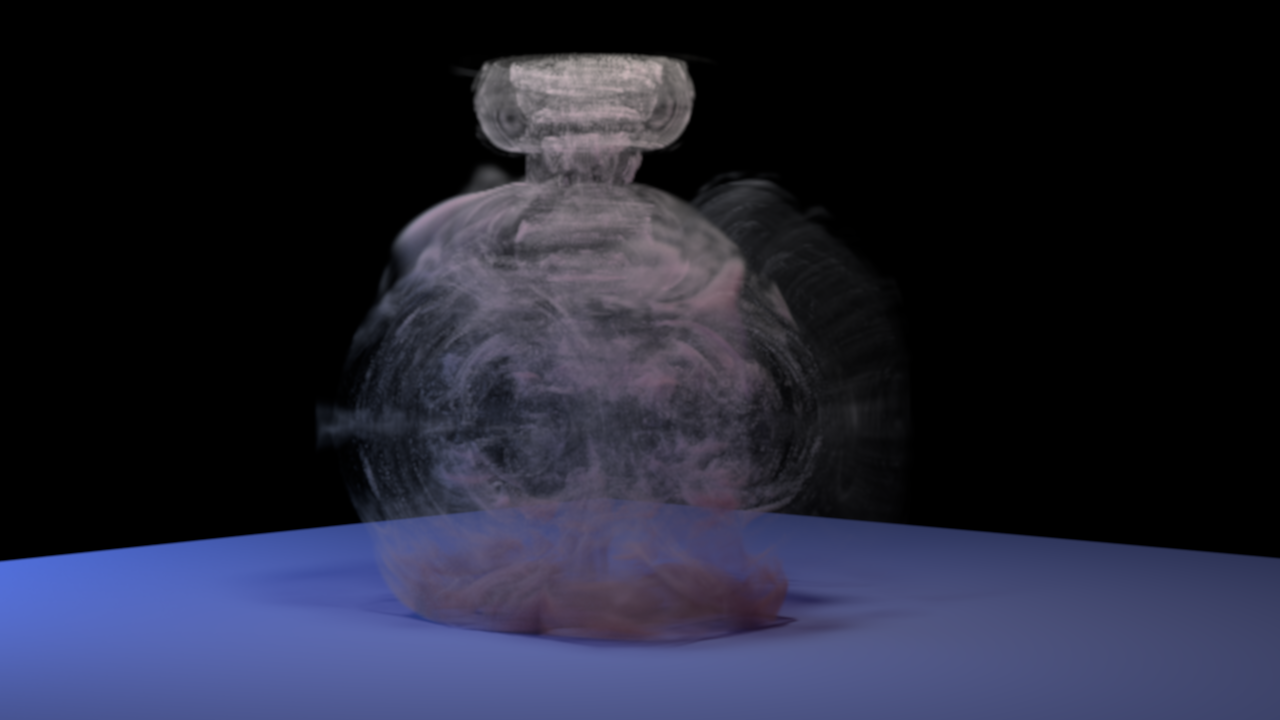
\includegraphics[width=\textwidth]{Figures/renders/plume0021.png}	
	\end{subfigure}
	%
	\begin{subfigure}[h]{0.5\textwidth}
		\centering
		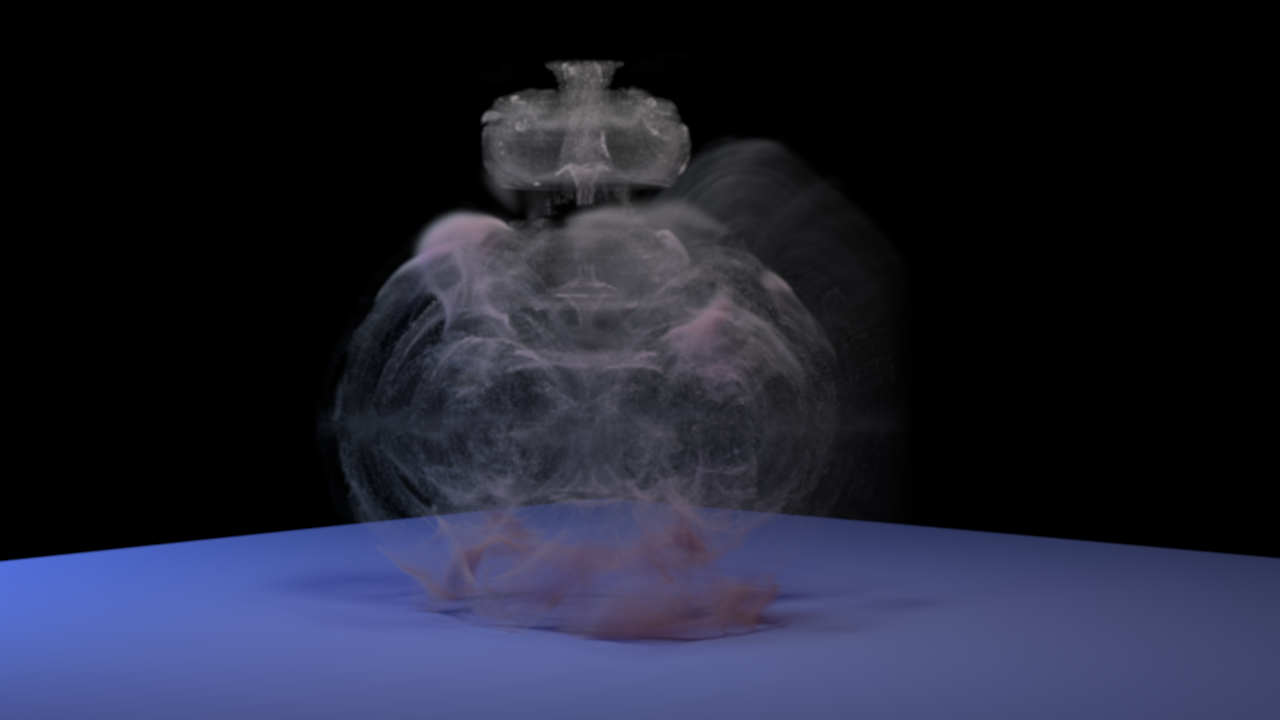
\includegraphics[width=\textwidth]{Figures/renders/plume0030.png}
	\end{subfigure}
	%
	\begin{subfigure}[h]{0.5\textwidth}
		\centering
		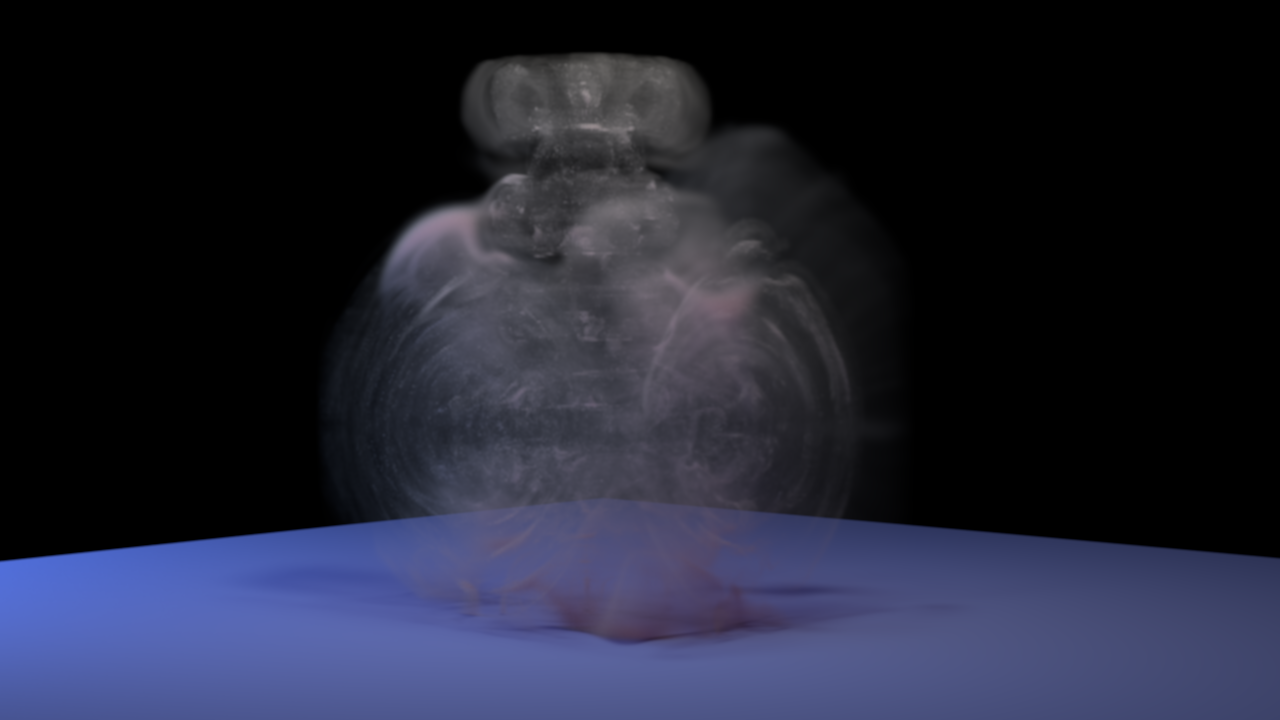
\includegraphics[width=\textwidth]{Figures/renders/plume0052.png}		
	\end{subfigure}
	%
	\begin{subfigure}[h]{0.5\textwidth}
		\centering
		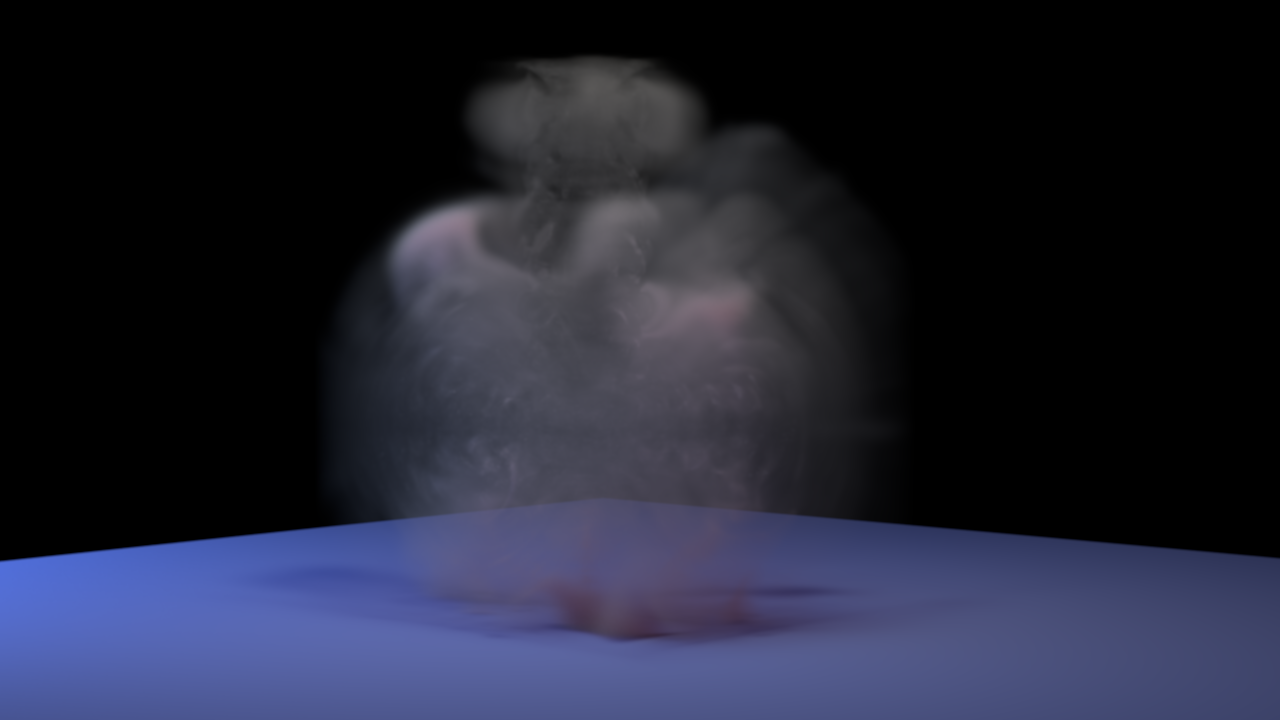
\includegraphics[width=\textwidth]{Figures/renders/plume0108.png}		
	\end{subfigure}
	\caption{An assortment of subspace fluid modes. \todo{ADJ: These are the coupled modes from the `scale' that are not as strong an analogy to the Chladni figures.}}
\end{figure*}
%%%%%%%%%%%%%%%%%%%%%%%%%%%%%%%%%%%%%%%%%%%

%%%%%%%%%%%%%%%%%%%%%%%%%%%%%%%%%%%%%%%%%%%
% ADJ: These are the more direct analogy to the Chladni figures.
\begin{figure*}
	\begin{subfigure}[h]{0.5\textwidth}
		\centering
		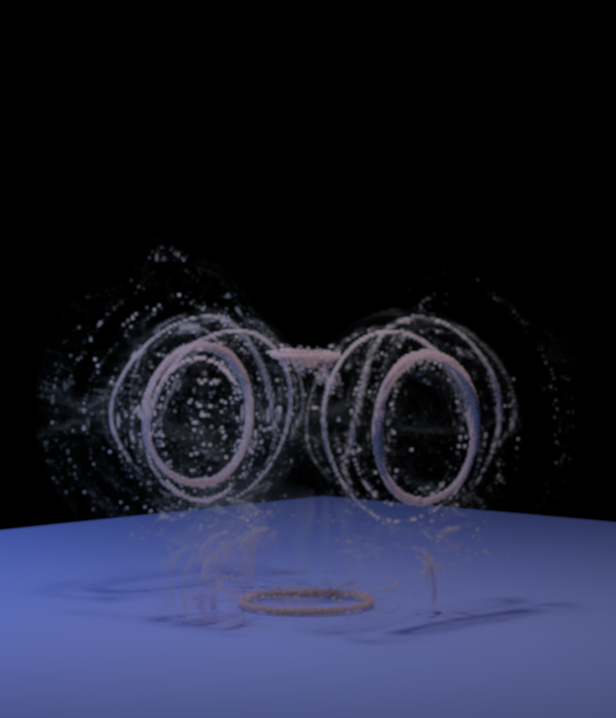
\includegraphics[width=\textwidth]{Figures/modes/plume0000.png}
	\end{subfigure}
	%	
	\begin{subfigure}[h]{0.5\textwidth}
		\centering
		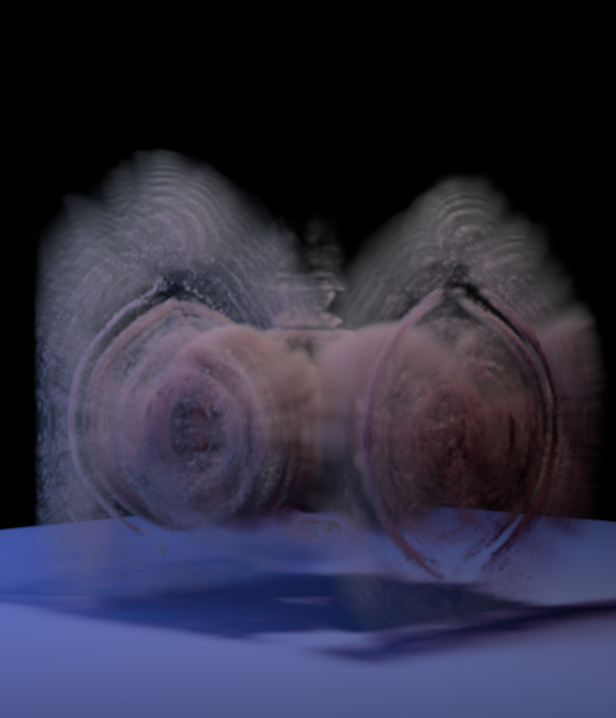
\includegraphics[width=\textwidth]{Figures/modes/plume0001.png}	
	\end{subfigure}
	%
	\begin{subfigure}[h]{0.5\textwidth}
		\centering
		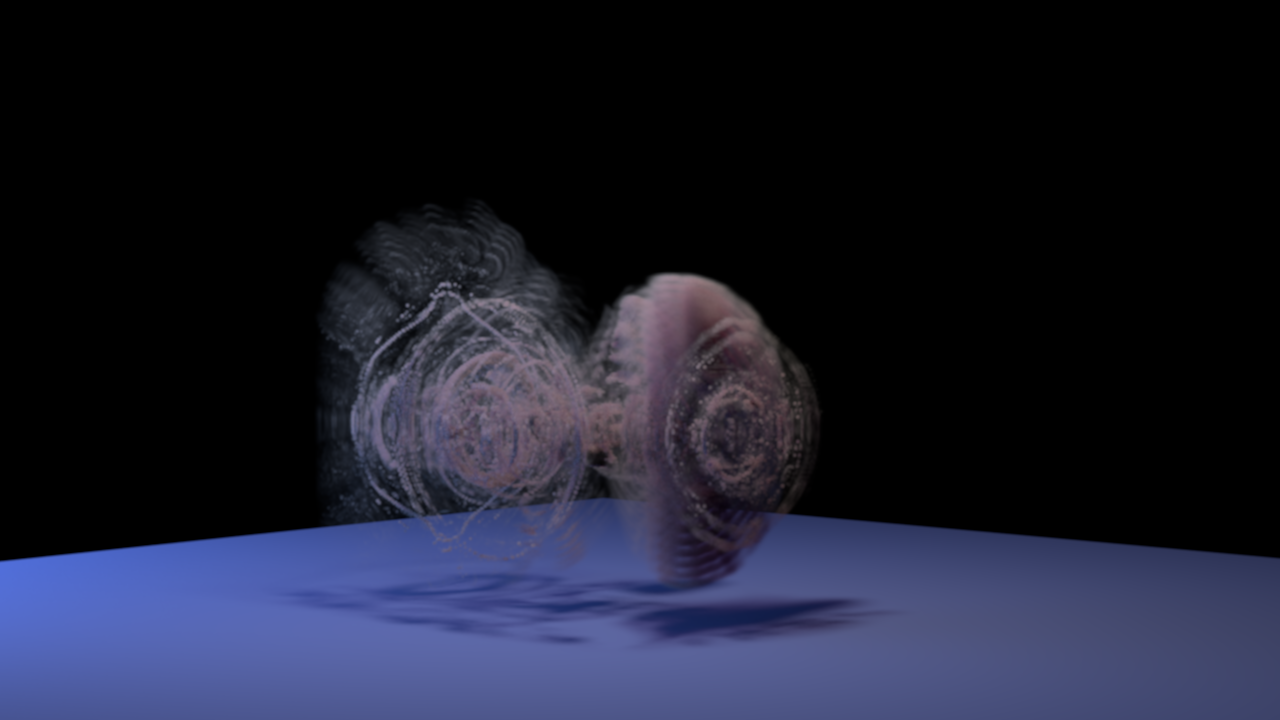
\includegraphics[width=\textwidth]{Figures/modes/plume0002.png}
	\end{subfigure}
	%
	\begin{subfigure}[h]{0.5\textwidth}
		\centering
		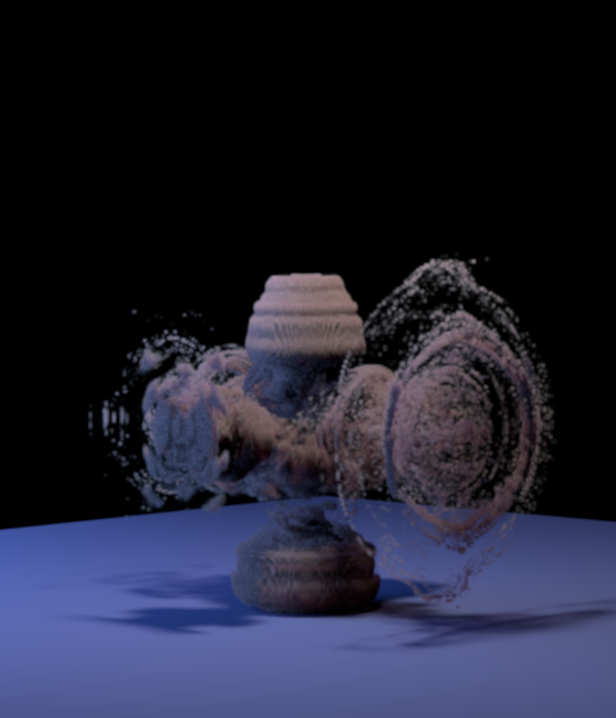
\includegraphics[width=\textwidth]{Figures/modes/plume0003.png}
	\end{subfigure}
	%
	\begin{subfigure}[h]{0.5\textwidth}
		\centering
		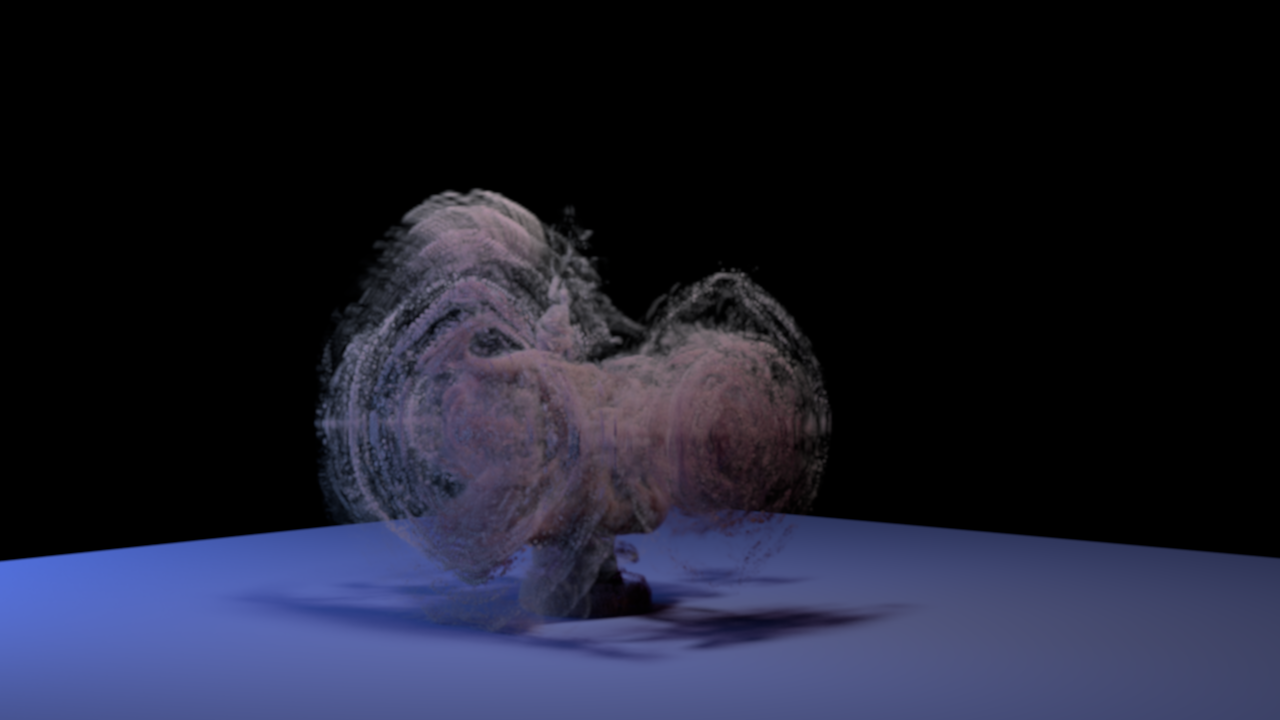
\includegraphics[width=\textwidth]{Figures/modes/plume0004.png}	
	\end{subfigure}
	%
	\begin{subfigure}[h]{0.5\textwidth}
		\centering
		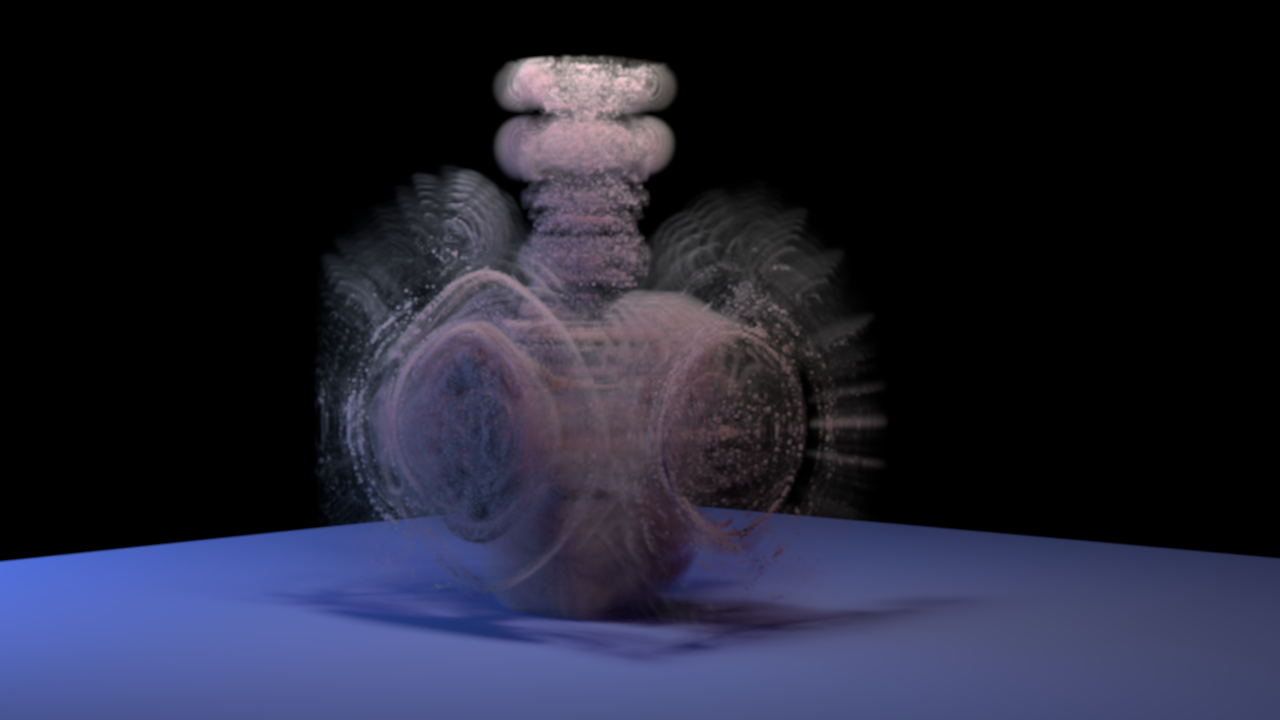
\includegraphics[width=\textwidth]{Figures/modes/plume0005.png}
	\end{subfigure}
	%
	\begin{subfigure}[h]{0.5\textwidth}
		\centering
		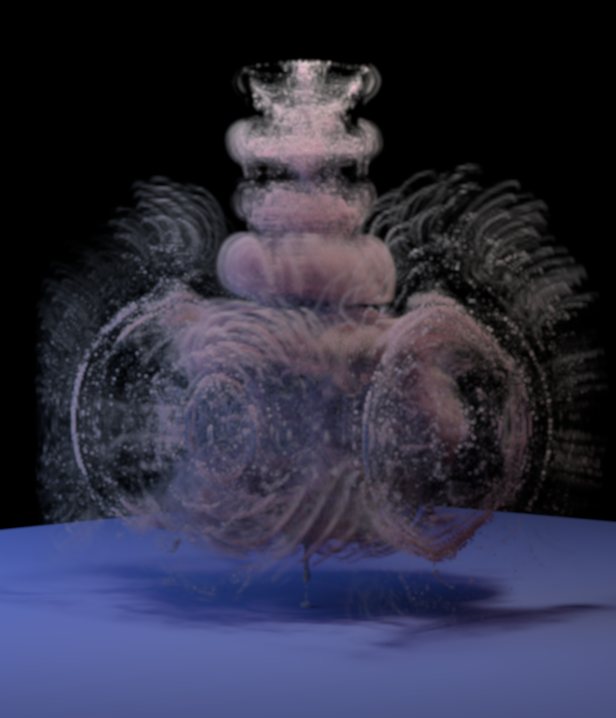
\includegraphics[width=\textwidth]{Figures/modes/plume0006.png}		
	\end{subfigure}
	%
	\begin{subfigure}[h]{0.5\textwidth}
		\centering
		\includegraphics[width=\textwidth]{Figures/modes/plume0007.png}		
	\end{subfigure}
	\caption{An assortment of subspace fluid modes. \todo{ADJ: These are the stronger analogy to the Chladni figures.}}
\end{figure*}
%%%%%%%%%%%%%%%%%%%%%%%%%%%%%%%%%%%%%%%%%%%

We can also step through the modes in a more physically faithful fashion. By gradually activating the modes one at a time without turning the previous ones off, the result when all $r$ are active converges to a physically accurate representation of the flow.

Other non-physical approaches are possible to explore based on the following observation. For each time step of the subspace re-simulation, when we perform the reconstruction phase, obtaining a full-space velocity field $\vv \in \R^{3N}$ from a reduced-order subspace vector $\qq \in \R^r$, we are simply taking a linear combination of the $r$ singular vectors using the corresponding coefficients given by the entries of $\qq$. Hence, the subspace vectors $q$ can be intuitively thought of as instructions for how to mix together the corresponding singular vectors with the appropriate weightings. Indeed, we can even identify a path $\varphi \colon [0, 1] \rightarrow S$, sampled at $T$ time steps $\varphi_1, \ldots, \varphi_T$, as determining the corresponding $T$ time steps of the full-space re-simulation, after reconstruction. 

%%%%%%%%%%%%%%%%%%%%%%%%%%%%%%%%%%%%%%%%%%%
\section*{Sonification}
We interpret the $r$ singular values $\sigma_1, \ldots, \sigma_r$ from the singular-value decomposition as characteristic frequencies. 

\begin{figure*}
	\begin{subfigure}[h]{0.5\textwidth}
		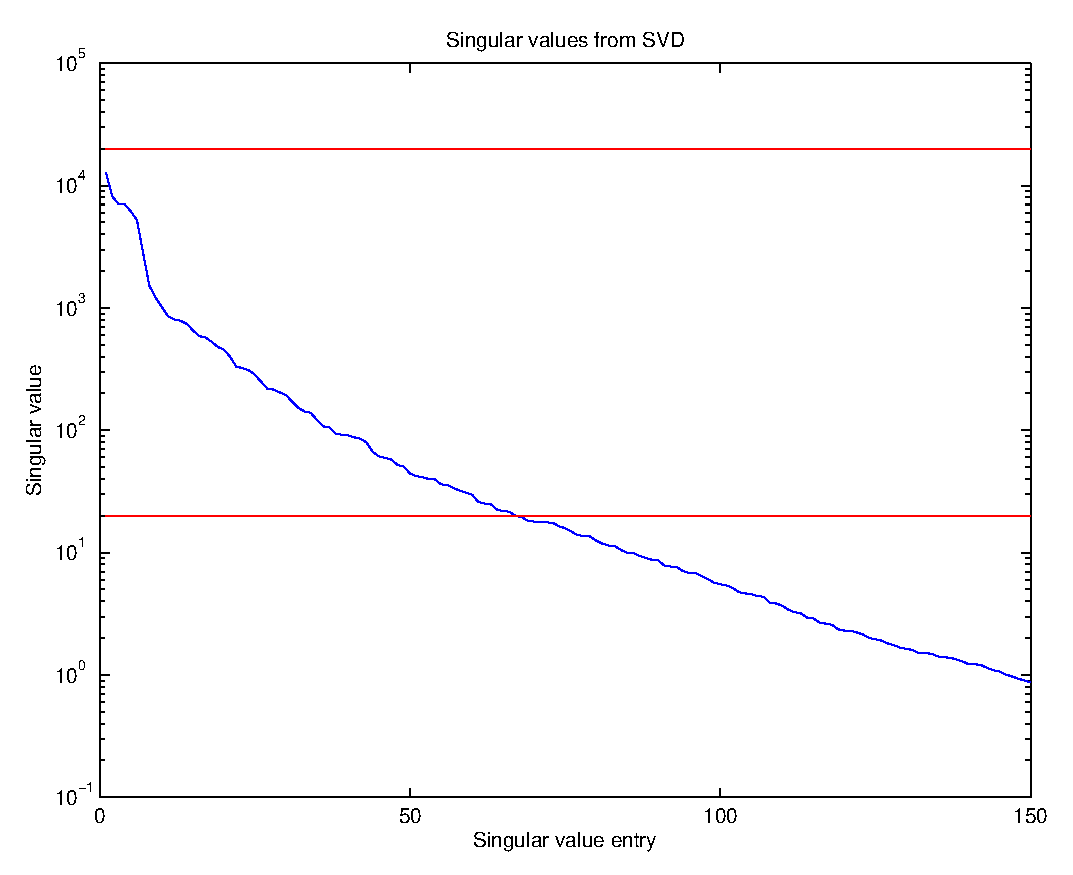
\includegraphics[width=\textwidth]{figures/singulars.eps}
		\caption{Singular values: r = 150} 
		\label{fig:singulars}
	\end{subfigure}
	%
	\begin{subfigure}[h]{0.5\textwidth}
		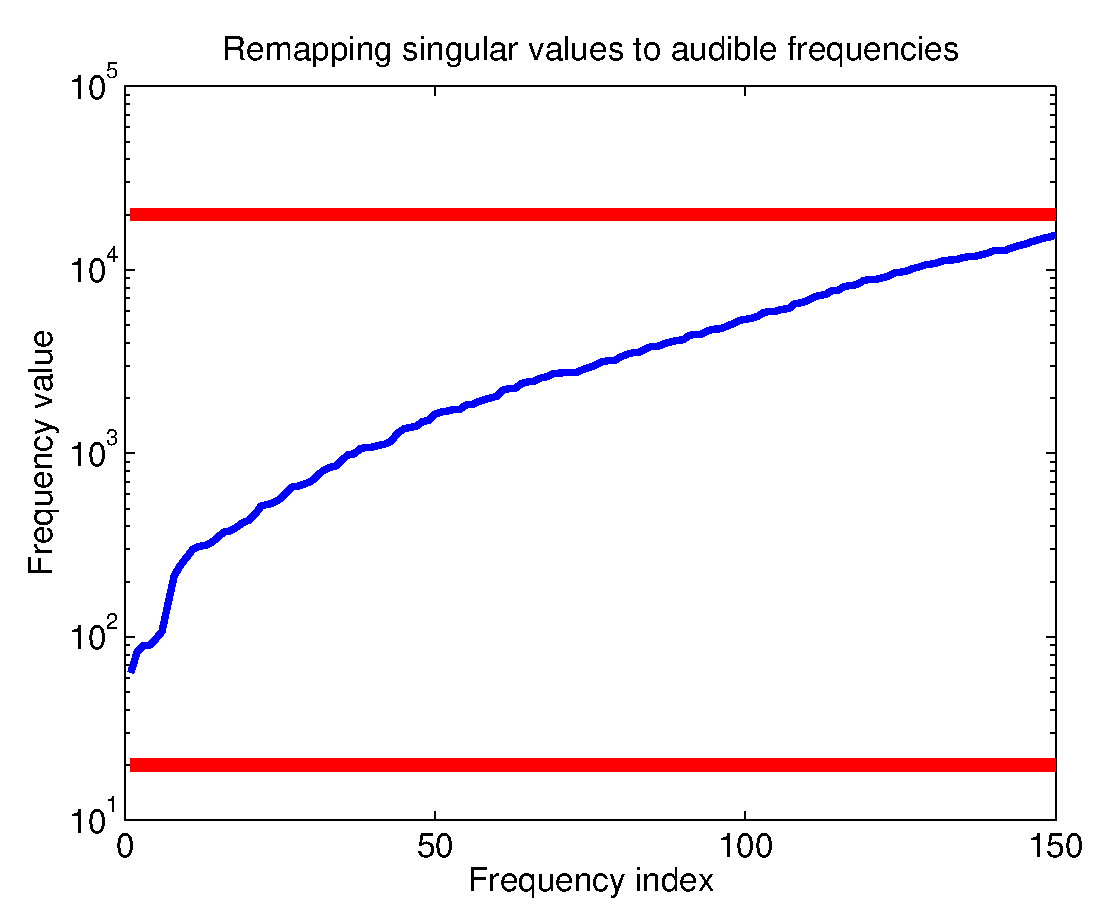
\includegraphics[width=\textwidth]{figures/remap_freqs.eps}
		\caption{Remapped frequencies: f = 64 Hz, s = 1.75}
		\label{fig:freqs}
	\end{subfigure}
	\caption{Singular values and their remapped frequencies. Note the logarithmic scale on both y-axes. The red lines on both plots indicate the bounds of the human audible frequency range.}
\end{figure*}

There are two immediate concerns about the raw data. Firstly, from Figure \ref{fig:singulars}, we see that the values range over approximately $4$ orders of magnitude, which is approximately $13$ octaves, and decrease to numbers less than $1$. However, the human audible dynamic range is generally considered to be from $20$ Hz to $20000$ Hz, which is only about $10$ octaves, and starts greater than $1$. Thus, we will have to rescale the octaves into an appropriate range and recenter the data. Secondly, starting from the principal singular value, the singular values are decreasing, whereas an audio spectrum increases from its fundamental frequency. Hence, we will have to invert the singular values. One way to proceed with a sensible mapping is to specify a desired fundamental frequency $f$ and an octave scaling $s$. Writing our audible frequencies as $f_1, \ldots, f_r$, we can define our mapping from singular values to audible frequencies as follows:

\begin{equation} 
\begin{aligned}
f_i &= f \cdot \left(\frac{\sigma_{i}^{-1}}{\sigma_{\textnormal{max}}^{-1}}\right)^{\frac{1}{s}} \\
&= f \cdot \left(\frac{\sigma_{\textnormal{max}}}{\sigma_i}\right)^{\frac{1}{s}}, \ i = 1, \ldots, r.
\end{aligned}
\end{equation}

The effect of this remapping can be seen in Figure \ref{fig:freqs}, where we have used a fundamental frequency $f = 64$ Hz and an octave scaling of $s = 1.75$. The spectrum now begins at the fundamental, $f = 64$ Hz, and ranges up to a maximum of approximately $15000$ Hz, an acceptable spread.

With an audible spectrum in hand, we now turn to the problem of choosing amplitudes for each individual frequency. These can be mapped from a corresponding subspace vector $\qq \in S$, as each of its $r$ components, $q_1, \ldots, q_r$ can be thought of as an amplitude for the $r$ corresponding frequencies $f_1, \ldots, f_r$. Care must be taken here too, as the overall sum of all the frequencies can exceed unity gain, which would lead to clipping. Mathematically, this means that we require the $L^1$ norm of $\qq$, $\lvert\qq\rvert_1 = \sum_{i=1}^{r}\lvert q_i \rvert$, to be at most $1$. A typical subspace vector $\qq$ may also contain negative components. However, these can simply be thought of as encoding a positive amplitude and a reversal of phase. The phase reversal can be discarded, as its perceivable effect is typically undesirable clicking artifacts.

With these considerations in hand, we design a mapping from a subspace vector $\qq$ to an amplitude vector $\aaa$ of unit $L^1$ norm as follows:
\begin{equation}
\begin{aligned}
a_i &= \frac{\lvert q_i \rvert}{\lvert\qq\rvert_1}, \ i = 1, \ldots, r.
\end{aligned}
\end{equation}
Given a sequence $(\qq_j)$ of vectors that describe a sampled trajectory $\qq_1, \ldots, \qq_T$ through the subspace $S$, we can either normalize each one of the corresponding amplitude vectors on an individual basis, or we can determine the subspace vector of maximum $L^1$ norm, $\qq_{\textnormal{max}}$, and normalize each amplitude vector based on $\lvert\qq_{\textnormal{max}}\rvert_1$. The effect of the former is a relatively uniform volume level, while the effect of the latter is usually a more variable volume envelope. Each approach has its own musical merit, depending on the compositional situation.

%%%%%%%%%%%%%%%%%%%%%%%%%%%%%%%%%%%%%%%%%%%
\section*{Synthesis}
With our mappings carried out, we can now produce sensible audible sound. The most basic technique to try is additive synthesis---namely, mixing together pure sine tones at the corresponding frequencies and amplitudes, creating an overall sound with a rich spectral content. With an instrument in hand that can produce the corresponding sound given a set of input amplitudes, a particular trajectory $\phi \colon [0, 1] \rightarrow S$ through the subspace, while retaining the same set of frequencies throughout time, determines a time-varying set of amplitudes, allowing the subspace evolution to dictate the time evolution of the sound. The overall effect is a subtle change in timbre, as the amplitudes of the various overtones fluctuate. 

Subtractive synthesis is also an interesting option. We start with a spectrally rich input sound, such as an impulse or broadband noise. We then create a filter bank of resonances at the appropriate set of frequencies, weighted in turn by the appropriate set of amplitudes. Some extra parameters must be addressed, as each resonant mode also is given a ring time for the mode to decay. The nature of the input sound also strongly influences the resulting timbre---broadband noise creates a more atmospheric effect, while impulses can create driving rhythmic textures. 

%%%%%%%%%%%%%%%%%%%%%%%%%%%%%%%%%%%%%%%%%%%
\section*{Time evolution}
Static sound, while interesting as a new timbre for a few seconds, eventually grows stale. Thus, we would like to capture the time evolution of the subspace trajectory as a dynamic sonic event. This can be achieved by cycling through the the sequence of amplitude vectors $\aaa_1, \ldots, \aaa_T$ corresponding to the subspace trajectory $\qq_1, \ldots, \qq_T$. Using subtractive synthesis, we can use the ring times to open and close the resonant frequencies in accordance to whether the corresponding modes are visually activated. As previously discussed, different trajectories through the subspace generated different sequences of amplitude vectors. The unfolding of these trajectories over time occurs on a micro-scale musically, but the choice of different possible abstract trajectories, and the shifting from one trajectory to another, is expressed on more of a meso- or even macro-level scale.

Experimentally, we have explored several different categories of subspace trajectories. The simplest is the original subspace re-simulation trajectory, which is faithful to the original simulation. original physics-based dynamics to update each timestep. It is also possible, however, to abandon the physics and simply choose a trajectory by other means. For example, starting from the same initial vector $\qq_1$ as in the original re-simulation, we can determine a trajectory simply by walking in a random direction at each time step, or walking along the surface of some abstract manifold $M \subset S$, such as a sphere. These lead both to unique visual and aural results. 

Since the the set of frequencies itself remains static over time, and only the amplitudes are changing, musically, it will also make sense to explore dynamically changing the pitch $f$ which was specified as the original fundamental frequency. This can be achieved simply by multiplying the entire spectrum by an interval, which will create a new fundamental without affecting the ratios between the partials. Alternatively, we could consider the original spectrum as a musical scale with which to compose melodies if we desire to compose more at the note scale.

%%%%%%%%%%%%%%%%%%%%%%%%%%%%%%%%%%%%%%%%%%%



%%%%%%%%%%%%%%%%%%%%%%%%%%%%%%%%%%%%%%%%%%%

% If you are only going to use a BibTeX database, from which all your cites will be
% taken and formatted consistently, use the following.

\bibliographystyle{plain}
\fontsize{10}{12}
\bibliography{mybib}

\end{document}